\documentclass[20 pts]{article}
\usepackage{xeCJK}
\usepackage{amsfonts}
\usepackage{amssymb}
\usepackage{amsmath}
\usepackage{bm}
\setCJKmainfont{SimSun}
\title{ターボ符号器における決定論的インタリーバの設計に関する研究} 
\author{Kwame Ackah Bohulu}
\date{2017/10/12}
\begin{document}
\maketitle

\newpage
\section{進捗状況}

\paragraph{[1].}
ターボ復号に応用するBCJRアルゴリズムのMATLAB実行に対するエラーを修正した。

\paragraph{[2].}

それぞれ1-1, 2-1, 3-1のエラーイベントを防止するようなインタリーバを設計した。
\paragraph{[3].}

1-1, 2-1, 3-1エラーイベントの組合を防止するようなインタリーバを設計した。
\section{今後の予定}
設計したインタリーバのビット誤り率性能の確認

\newpage
\begin{center}
\begin{figure}
		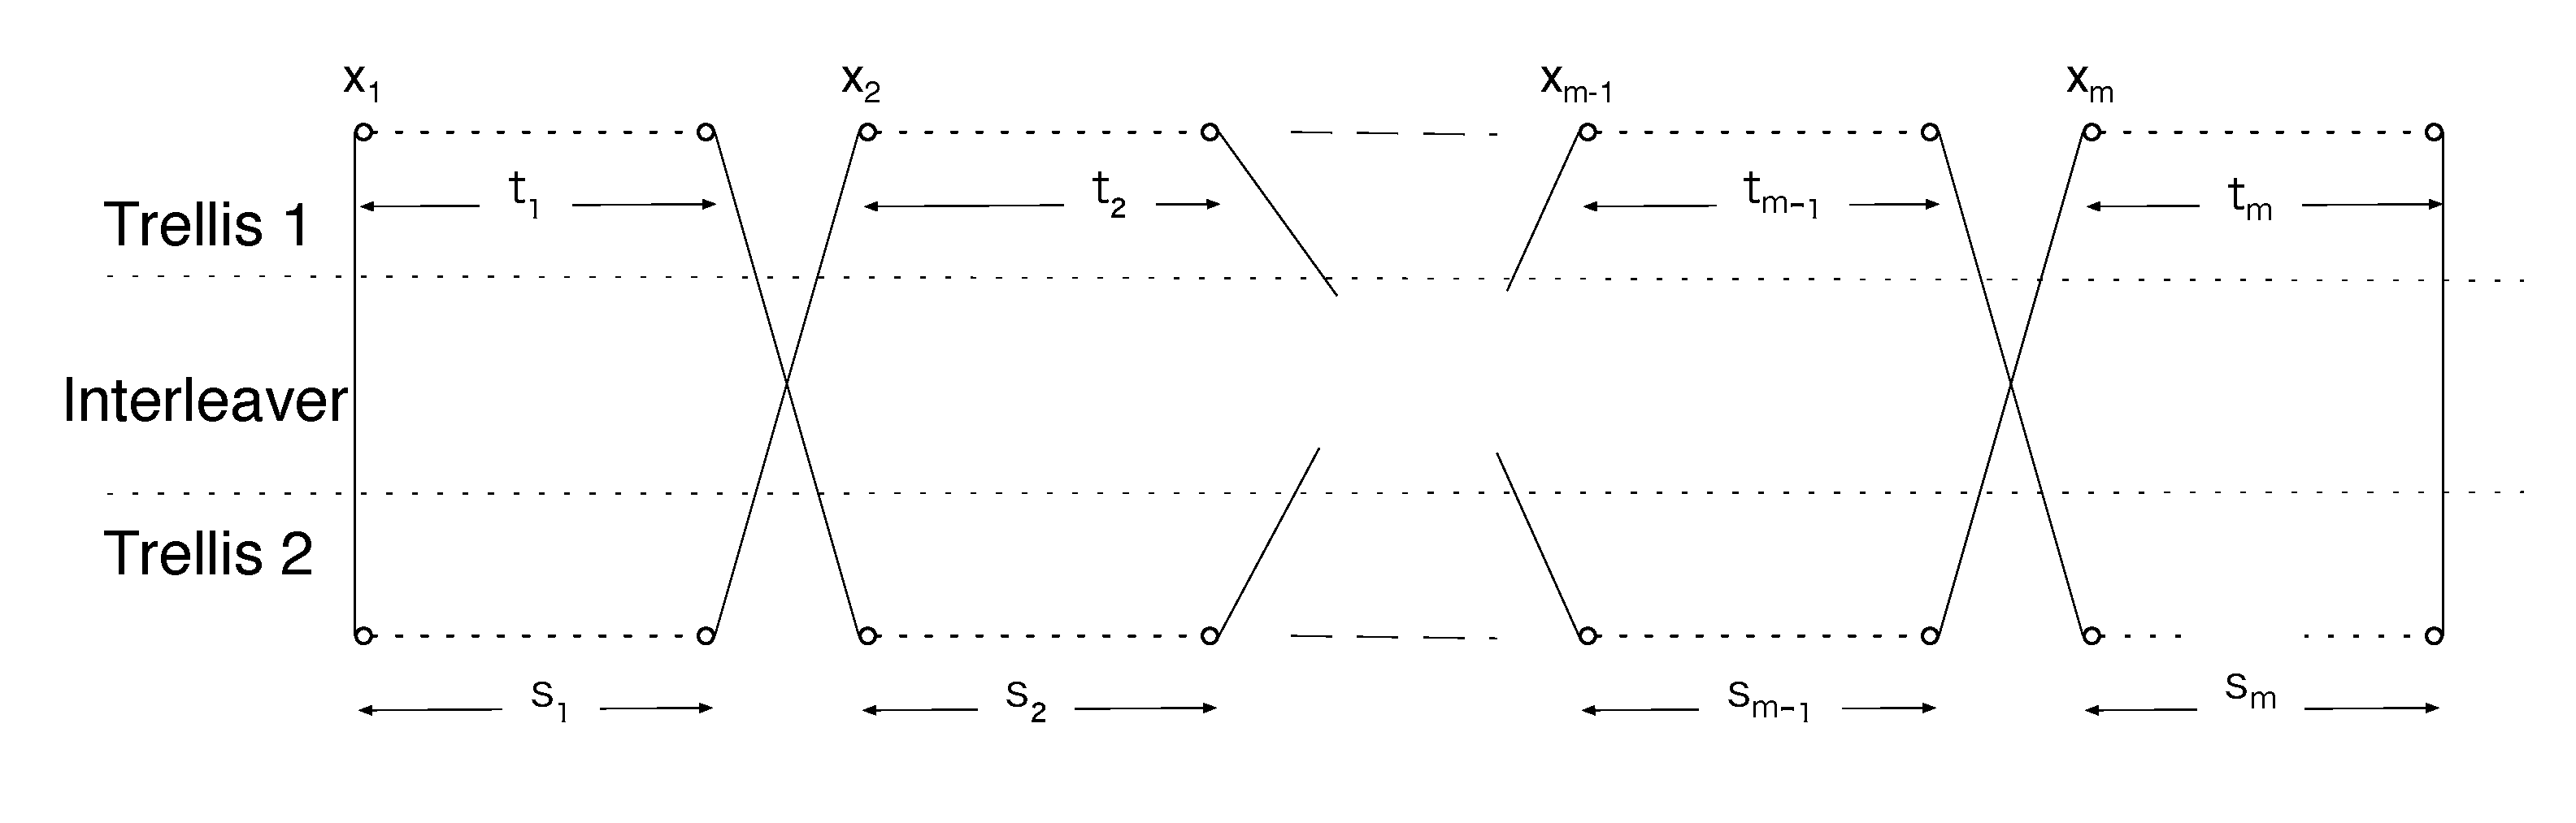
\includegraphics[width=\textwidth]{weight2m.pdf}
		\caption{a$\tau$-seperated weight 2m error event}
		\end{figure}
	\end{center}
	
	\begin{center}
\begin{figure}
		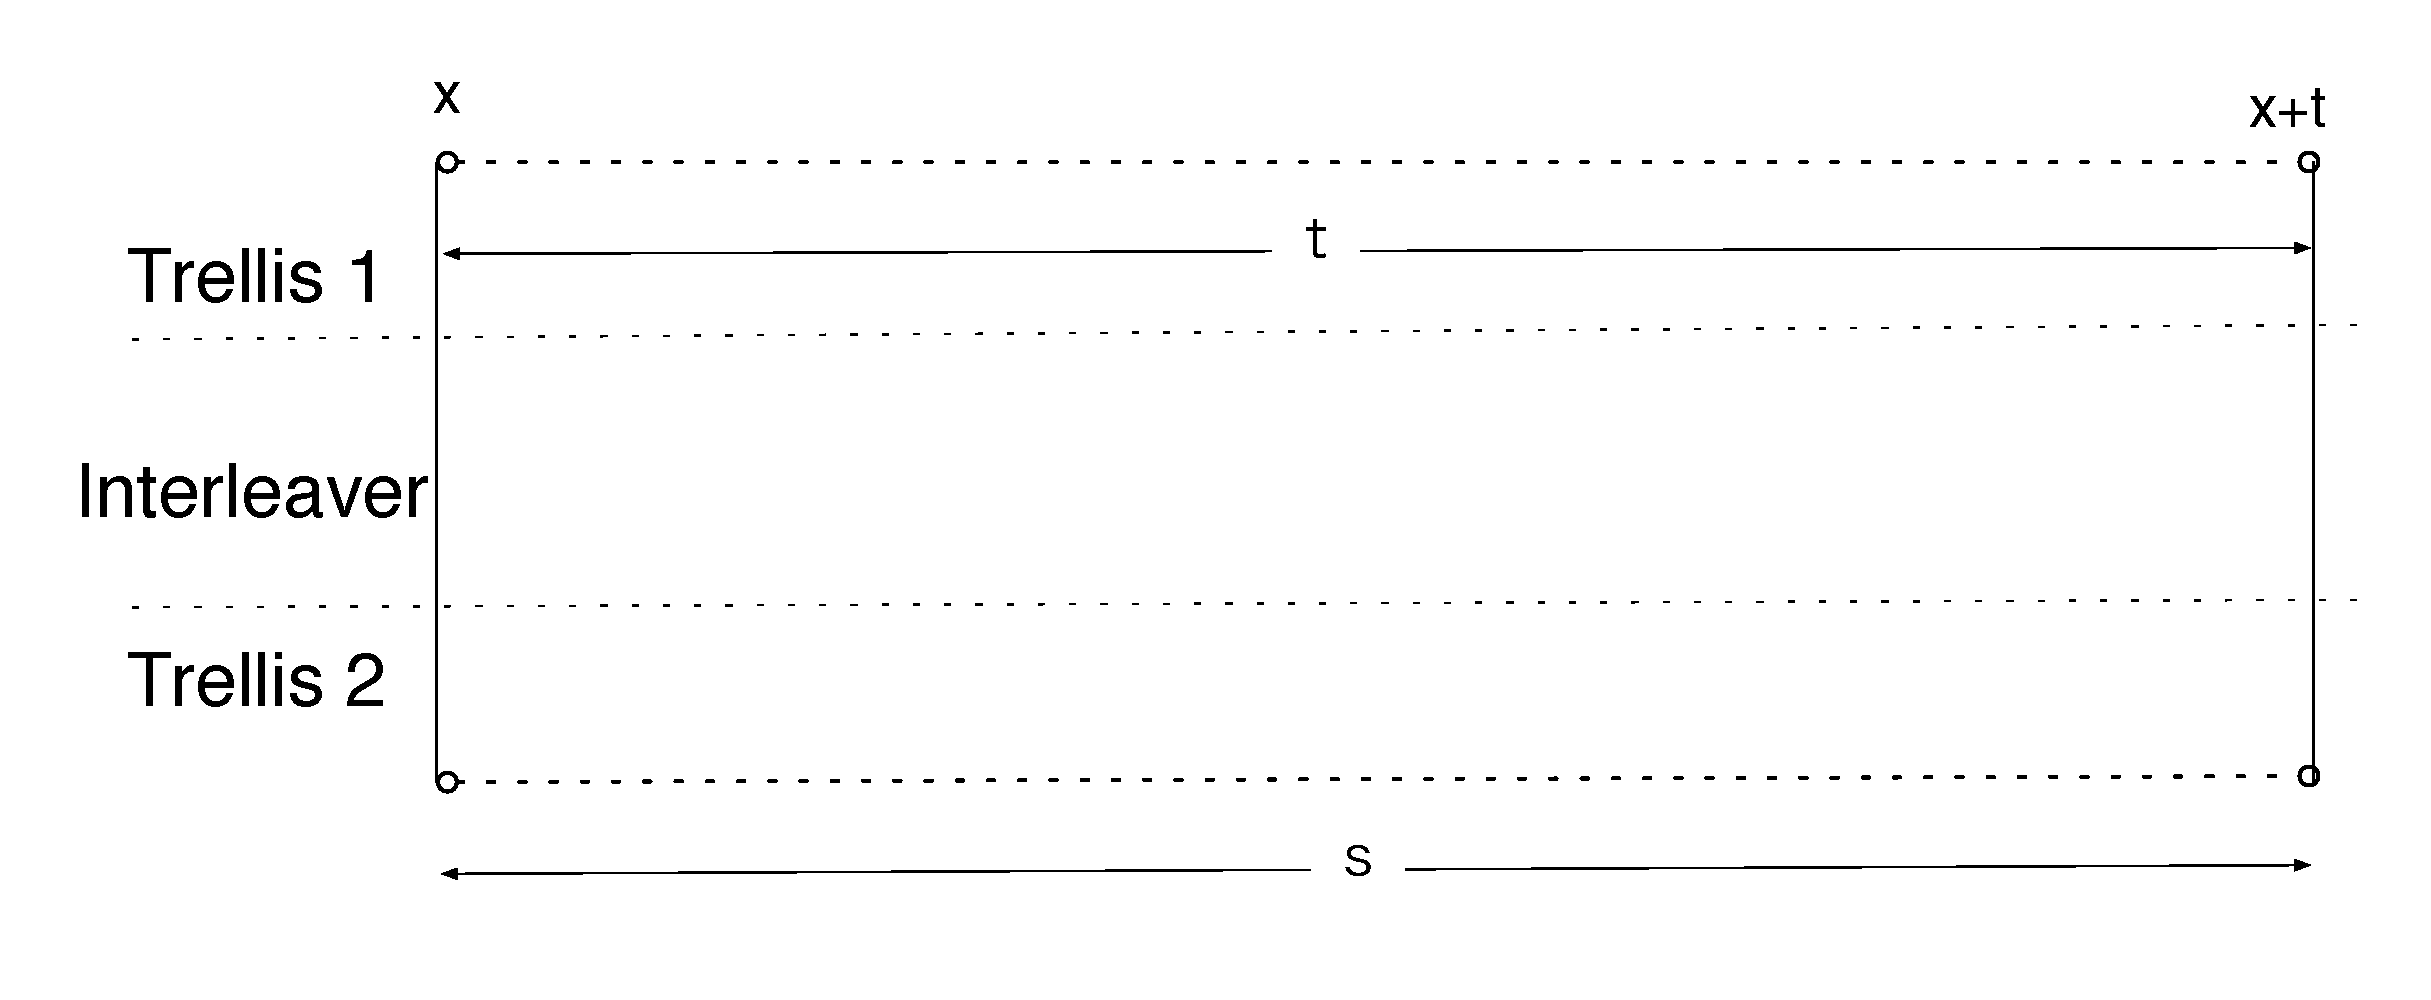
\includegraphics[width=\textwidth]{weight2.pdf}
		\caption{a$\tau$-seperated weight 2 error event}
		\end{figure}
	\end{center}
	
	\section{Interleaver Design}
\begin{equation}
\Pi_{\mathbf{L}_n}(i) \equiv bi  \mod N, \ 0 \leq i \leq N
\label{linear}
\end{equation}
sは以下の式で計算する。
\begin{equation}
\begin{split}
s&=\Pi_{\mathbf{L}_n}(x+t)-\Pi_{\mathbf{L}_n}(x)\\
&=b(x+t)-b(x) \mod N\\
&=bt \mod N
\label{three}
\end{split}
\end{equation}
符号語の重みは以下の式で計算する。
\begin{equation}
d_{(t_i,s_i)}=6+\Bigg( \frac{ \left|t_i\right|}{\tau} + \frac{ \left|s_i\right|}{\tau} \Bigg)w_o 
\label{four}
\end{equation}

式 (\ref{three}) を式 (\ref{four}) 入力し、$t$ を $\tau$ に書き換えると
\begin{equation}
d_{(t_i,s_i)}=6+\Bigg( 1+ \frac{ b\tau \mod N}{\tau} \Bigg)w_o 
\label{five}
\end{equation}
以下の条件を満たすbを使用する。
\begin{equation}
( (b\tau \mod N )\mod \tau ) \neq 0
\label{six}
\end{equation}
sを大きくするbを選択方法は以下で説明する。

\paragraph{1.}  (\ref{six}) の条件を満たすi番目のbを選択して、$(1+D^{t\tau})(D^u) ,0\leq u\leq N-\tau, t=1$の形を持つエラーイベントに対するsを(\ref{three})で計算する。
\paragraph{2.} 符号語の重みを (\ref{four}) で計算し、min $d_{(t_i,s_j)}$を保存する。
\paragraph{3.}すべてのbに対する min $d_{(t_i,s_j)}$ を保存して、 max(min $d_{(t_i,s_j)}$)に関するbを選ぶ。


\end{document}